\documentclass[prb,preprint]{revtex4-1} 
\raggedbottom
\usepackage{amsmath}
\usepackage{amsfonts}
\usepackage{graphicx}

\begin{document}

\title{On The Attenuation Coefficient for\\ 1.33 MeV Gamma-Rays from a $^{60}$Co Source}

\author{Ryan S. Morshead}

\affiliation{Department of Physics, California State Polytechnic University}

\date{\today}

\begin{abstract}

Utilizing a photomultiplier tube (PMT) along with a scintillating NaI crystal, the attenuation coefficient, $\mu$, of a beam of gamma-rays emitted by a $^{60}$Co source was determined. This was accomplished by passing this beam through a collimator and an absorbent, where it would finally impact the scintillator. By counting the current pulses produced by the PMT with a multi-channel analyzer (MCA) over a fixed time period, $\mu$ could be calculated from the data which was gathered. Given that the density of lead is 11.3 g/cm$^3$, and the density of aluminum is 2.7 g/cm$^3$, $\mu$, as found from lead, was $0.0501\pm0.0004$ cm$^2$/g, while its value as found from aluminum was $0.0552\pm0.0004$ cm$^2$/g. $\mu$ from lead and aluminum are both in disagreement with what can be extrapolated from data collected by The National Institute of Standards and Technology (NIST). It was determined that the NIST data gives $\mu$ to be 0.0566 cm$^2$/g for lead and a 0.0535 cm$^2$/g for aluminum\cite{NIST}.

\end{abstract}


\maketitle


\section{Introduction}

Radiation physics and chemistry flourished at the end of the 20th century; Wilhelm Conrad Rontgen made his sensational discovery of X-rays in 1895 which was soon followed by Henri Becquerel's discovery of radioactivity and by J. J. Thomson's proof of the independent existence of negative electrons of small mass \cite{henri}. Then Marie and Pierre Curie discovered the radioactive elements polonium and radium, and Paul Villard made the first detailed observations of gamma rays\cite{curie,V1}. Though Paul Villard is almost forgotten today by the scientific community, he is given credit for having discovered gamma-rays. His discovery is almost never discussed in any detail, as one might say he stands in the shadow of giants.

It was on May 18$^{th}$ that Villard demonstrated that radium emits rays which are non-deviable under the influence of magnetic fields and are capable of penetrating dense objects\cite{V2}. These new rays, said Villard, were different from the radium rays observed so far. He went on to suggest that the extremely penetrating rays, were similar to the X-rays previously observed by Rontgen and thus he claimed they were a form of X-ray\cite{V2}.

This paper seeks to quantify the penetrating capabilities of gamma rays which Villard noted in his first observations of gamma-rays.

\newpage

\section{Experimental Design}

Detecting $1.33$ MeV gamma-rays from a Co source for the purpose of measuring their attenuation was achieved here by utilizing a PMT along with a scintillating NaI crystal. As is shown by Fig \ref{ExpFig}, a beam of gamma-rays emitted by a $^{60}$Co source passes through a collimator, an absorbent, and finally impacts the NaI crystal. In the arrangement shown, counting the current pulses produced by the PMT with an MCA over a fixed period of time allows for the attenuation of the photons to be measured. 

\begin{figure}[h!]
\centering
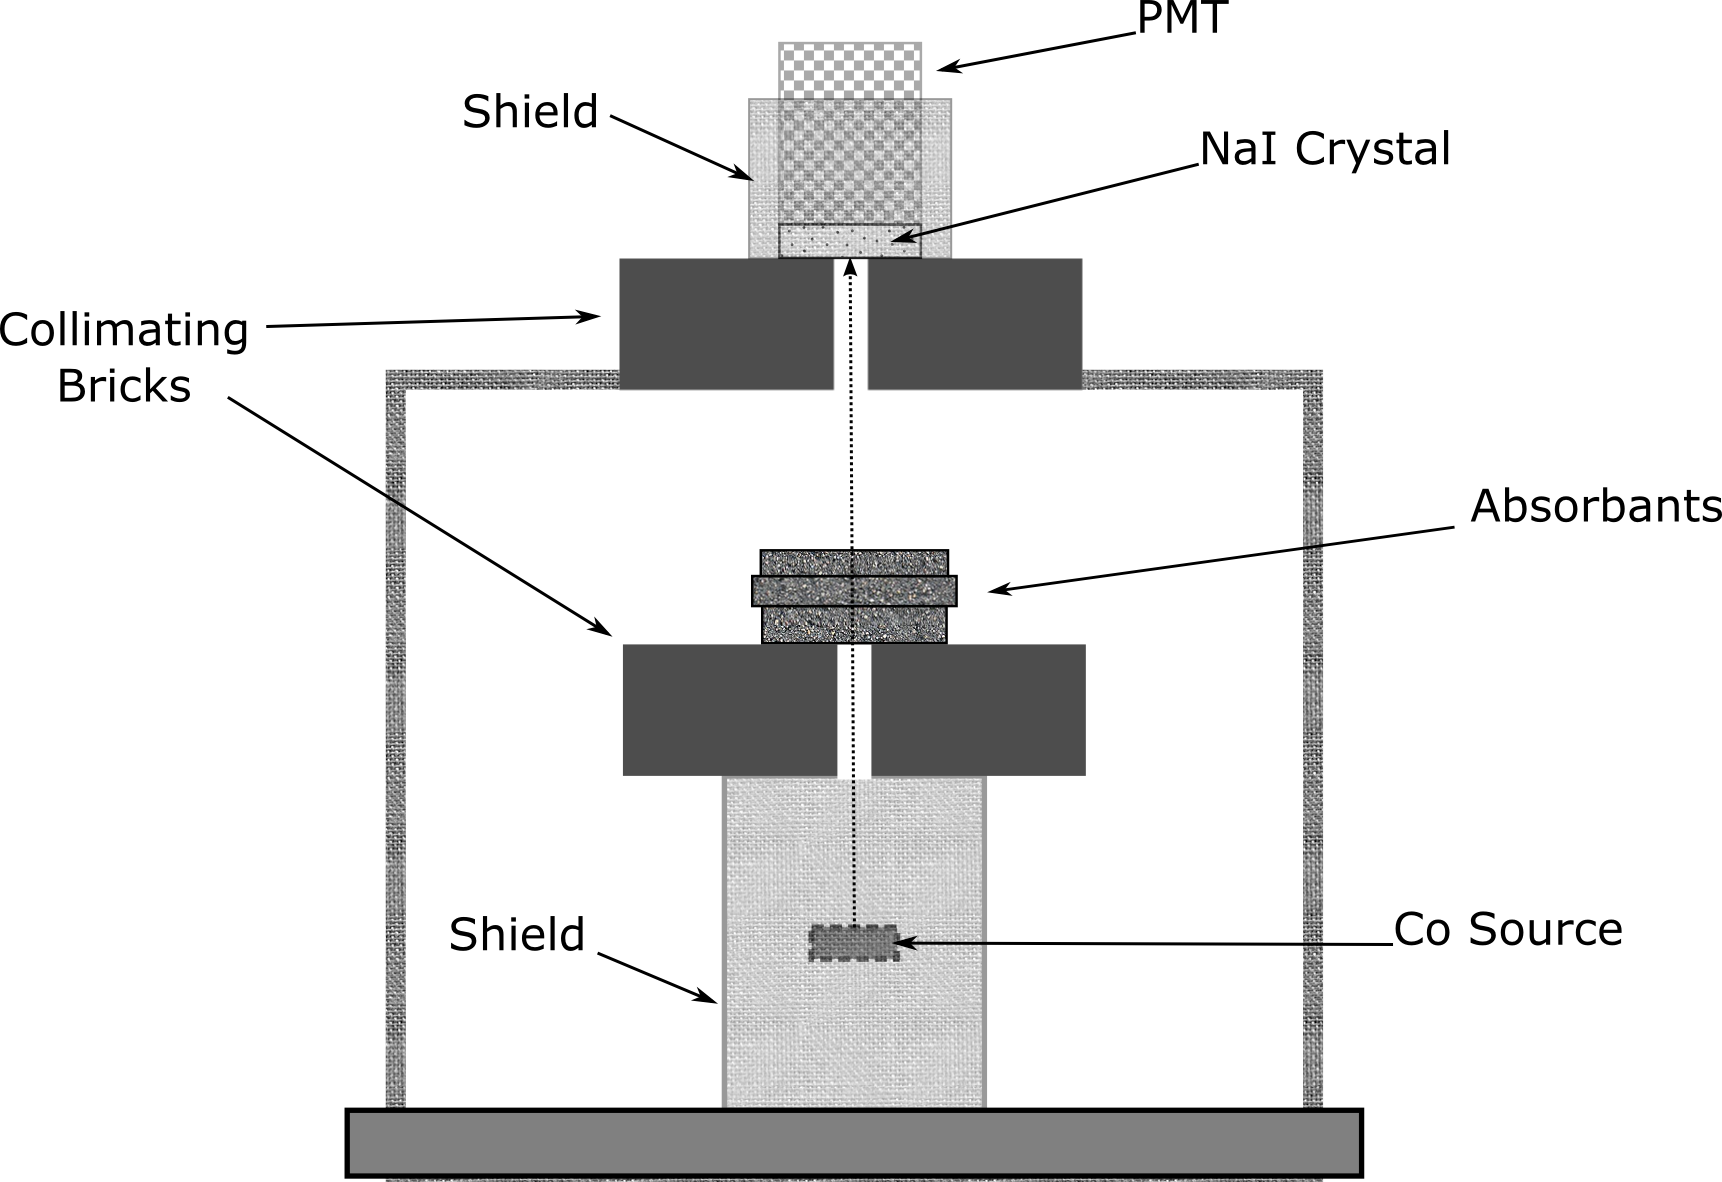
\includegraphics[width=.85\textwidth]{ExpFig.png}
\caption{The experimental apparatus which includes a PMT and scintillation crystal for gamma-ray detection.}
\label{ExpFig}
\end{figure}

The $^{60}$Co source which was used decays to $^{60}$Ni. To do this $^{60}$Co undergoes a 0.31 MeV $\beta$ decay or a 1.48 MeV $\beta$ decay. These are shown in Fig \ref{CoDecay}. Through either of these decays, the resulting $^{60}$Ni is found in an excited state and will emit gamma-rays with 1.17 MeV and 1.33 MeV or 1.33 MeV respectively.

\begin{figure}[h!]
\centering
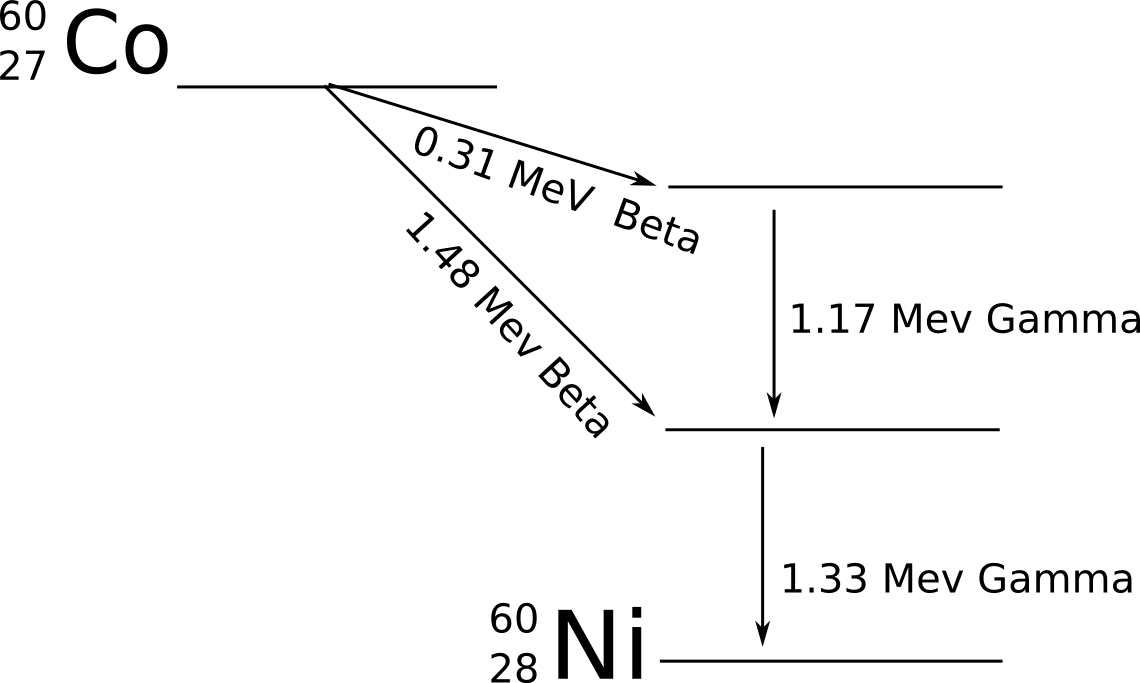
\includegraphics[width=.8\textwidth]{CoDecayScheme.png}
\caption{The $^{60}$Co to $^{60}$Ni decay scheme showing the resulting 1.17 MeV and 1.33 MeV gamma-rays.}
\label{CoDecay}
\end{figure}

By increasing the thickness or the density of the absorbents there will be a drop in the photon flux at the PMT.  This results from the interaction of photons with particles in the material. Unlike charged particles, in this context, if photons from the source interact with the material, the results are either the photoionization of atoms, Compton scattering, or electron positron pair production from photons higher than 1.022 MeV. The first and last possibilities result in the energy of the photon being lost to the material, while the second results in the photon being deflected out of the collimated beam.

If we consider a beam of gamma-rays passing through matter with some intensity $I$, measured in photons per second. In moving a small distance $dx$ there will be a corresponding reduction in intensity $dI$. If the probability per unit of distance of losing a photon by the previously described means is $\alpha$, then we may write the decrease in intensity as
\begin{equation}\label{dI}
dI=-I \alpha dx.
\end{equation}
Here $\alpha$, known as the absorption coefficient, is dependent on the energy of the gamma-rays and on the density of the material they are passing through. Then, by solving the differential equation for $I$ we find through the expression
\begin{equation}\label{I}
I(x)=I_0e^{-\alpha x},
\end{equation}
an exponentially decreasing intensity which is dependent on $x$, $\alpha$, and the initial intensity $I_0$. By defining the range, $\lambda$, to be the mean distance traveled before absorption as well as the distance traveled before the intensity is reduced to $e^{-1}$ we can show that
\begin{equation}
\lambda=1/\alpha.
\end{equation}

Though this is a useful equation, the constants are not all that pertinent in the context of nuclear physics as materials are not typically defined by their thickness, $x$, but by the equivalent matter, $\xi$, which has units of g/cm$^2$. $\xi$ is defined as $\rho x$ which implies that $\xi$ is the mass of a cylinder with a base area of 1 cm$^2$ and a height $x$, where $x$ in this case will be the thickness of the absorbent. Because $\xi$ is proportional to the number of atoms a photon will encounter, and because that number dictates how likely it is for a photon to be absorbed, $\xi$ is a useful characteristic of a material. In order to include $\xi$ in Eq \eqref{I} we multiply the term in the exponent by $\rho/\rho$ bringing factors of $1/\rho$ to $\alpha$ and of $\rho$ to $x$. Then, by recognizing $\rho x$ to be $\xi$ we can rewrite Eq \eqref{I} as
\begin{equation}
I(x)=I_0e^{-(\alpha/\rho)\xi},
\end{equation}
where we will then define the mass attenuation coefficient as $\mu=\alpha/\rho$ to further alter $I(x)$ and define it as
\begin{equation}
I(x)=I_0e^{-\mu\xi}.
\end{equation}
$\mu$ has the benefit of being relatively independent of the characteristics of the absorbent material and thus can be said to be an attribute of the photon energy. $\alpha$ on the other hand is dependent on both the material and the photon energy making it difficult to distinguish between how they influence $\alpha$ individually. As a result $\alpha$ is an unfavorable variable to use.

In order to determine $\mu$ for the 1.33 MeV gamma-rays emitted by our $^{60}$Co source we use the intensity of the emitted photons for different values of $x$. With the recorded thicknesses and intensities we then fit the data to a linear curve
\begin{equation}\label{ln(I)}
ln(I(x))=ln(I_0)-\alpha x,
\end{equation}
which is described by taking the natural log of Eq \eqref{I}. In this form $-\alpha$ becomes the slope of the graph while $ln(I_0)$ will become its y-intercept. As a result determining the slope of the line which best fits the data using a weighted least squares optimization will determine an experimental value for $\alpha$ and then, with a known value for the density of the absorbent, we can determine $\mu$.

Here, two different absorbents, lead and aluminum, are used to determine the common attenuation coefficient for the 1.33 MeV gamma-rays being emitted by a $^{60}$Co source. In both cases the same methodology is used. This approach begins by measuring background counts. The background measurement is then subtracted from the total number of gamma-rays recorded by the PMT as the thickness of the absorbent increases. The corrected counts, $N$, and the associated $x$'s, are then plotted against each other to produce an exponential relationship.  As a result of the fact that all $N$'s are recorded in a set time period they are directly proportional to the intensity. This allows us to apply Eq \eqref{ln(I)} and take the natural log of $N$ to linearize that data. A linear least squares optimization of $\alpha$ and $ln(N_0)$ is then applied to this altered data, where $N_0$ is the counts with no absorbent present. With this information $\mu$ can then be calculated given known values for the density of aluminum and lead. To ensure that our results are accurate they are compared against the values found by NIST.



\newpage

\section{Results and Analysis}

Using the MCA a 1 minute live time spectrum for the decay of $^{60}$Co was recorded without absorbents present. This spectrum is shown in Fig \ref{0Plate}. The following analysis focuses on the 1.33 MeV peak. Using the counts contained inside the 1.33 MeV peak we estimate how long it will take to acquire 10,000 counts and then maintain this integration time for the remainder of the experiment. We then record, $N_m$, the measured counts at different thicknesses of the two absorbents. For lead we stack 1, 2, 3, 4, 5, 6, and finally 8 absorbing plates over the collimating brick, while for aluminum we add plates until the counts have decreased from their initial amount by a factor of 8. To measure the background counts, $N_b$, we introduce approximately 5 inches of lead shielding to the photon path and record counts. $N_b$ is then subtracted from all $N_m$ to give us our net counts $N_{Pb}$ and $N_{Al}$ for lead and aluminum respectively. Under these conditions we find $N_b$ to be $20\pm4.5$. Using a thickness of approximately 5 inches, Eq \eqref{ln(I)}, and our measured value for $\alpha$ shown in subsection A of section III, we can say that our count contamination from the source is approximately $0.0008 N_0$ because of our extended integration time. By our previous procedure $N_0$ is 10,000 counts, thus showing that our background contamination lies within two standard deviations of our background uncertainty. From this we can then say that the corrected counts from lead, $N_{Pb}$, and from aluminum, $N_{Al}$, which are shown in Table \ref{Trials}, accurately reflect the true counts from our  $^{60}$Co source. 
\begin{figure}[h!]
\centering
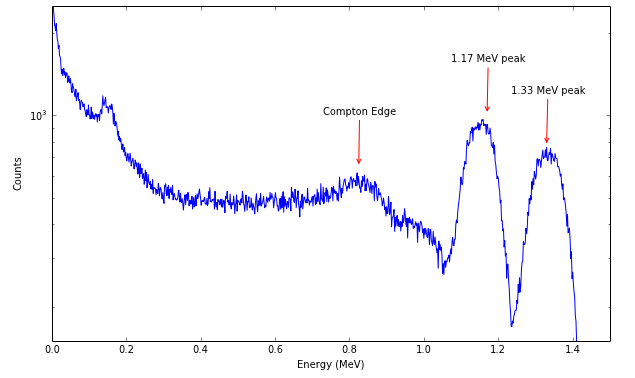
\includegraphics[width=.8\textwidth]{Spectra.png}
\caption{The unobstructed spectrum for $^{60}$Co used to determine the fixed integration time.}
\label{0Plate}
\end{figure}

\newpage

\begin{table}[h!]
\centering
\caption{Absorbent thicknesses, corrected counts, and error in the associated counts for lead (denoted as Pb) and aluminum (denoted as Al).}
\begin{ruledtabular}
\begin{tabular}{c c c c c c p{4 cm}}
$x_{Pb}$ (cm) & $N_{Pb}$ &$x_{Al}$ (cm) & $N_{Al}$\\
\hline
0        & $9669\pm98.5$ & 0      & $10021\pm100.2$\\
0.541 & $7210\pm85.1$ & 1.31 & $8422\pm91.9$\\
1.07   & $5083\pm71.6$ & 2.62 & $6846\pm82.9$\\
1.60   & $3976\pm63.4$ & 3.93 & $5543\pm74.6$\\
2.12   & $2942\pm54.6$ & 5.24 & $4762\pm69.2$\\
2.64   & $2168\pm47.0$ & 6.55 & $3645\pm60.5$\\
3.20   & $1640\pm41.0$& 7.86 & $3106\pm55.9$\\
4.24   & $829\pm29.5$  & 9.17 & $2564\pm50.8$\\
          &                          & 10.5 & $2223\pm47.4$\\
          &                          & 11.9 & $1797\pm42.6$\\
          &                          & 13.1 & $1501\pm39.0$\\
          &                          & 14.1 & $1134\pm34.0$\\
          &                          & 15.7 & $1001\pm32.0$\\
          
\end{tabular}
\end{ruledtabular}
\label{Trials}
\end{table}

\newpage

\subsection{Lead}

From the data in Table \ref{Trials}, $\alpha$ was determined to be $0.566\pm0.005$ cm$^{-1}$ using a fit function of the form of Eq \eqref{ln(I)} and the least squares method previously described. From this value we find $\lambda$ to be $1.77\pm0.02$ cm and $L_{1/2}$, the distance at which the intensity is reduced by a factor of 1/2, to be $1.22\pm0.01$ cm. Given that the density of lead is 11.3 g/cm$^3$, $\alpha$ also gives us a value for $\mu$ which is $0.0501\pm0.004$ cm$^2$/g. Though NIST has no specific value for the attenuation coefficient at 1.33 MeV for lead, data extracted from Fig \ref{LeadMu} gives an accepted value of 0.0566 cm$^2$/g showing that our value is in disagreement with what can be extrapolated from NIST's data \cite{NIST}.

\begin{figure}[h!]
\centering
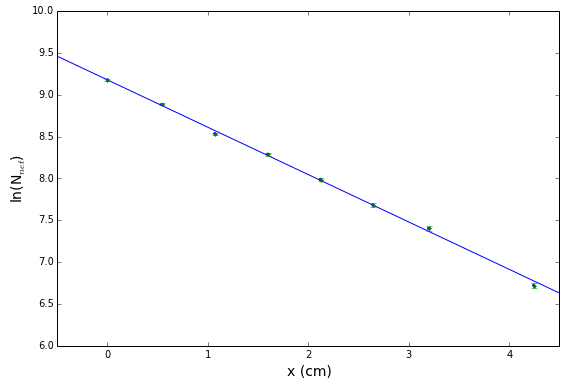
\includegraphics[width=.8\textwidth]{LeadFit.png}
\caption{The least squares optimization of $\alpha$ and $ln(I_0)$ based on absorbent thickness and the natural log of the intensity.}
\label{LeadFit}
\end{figure}

\begin{figure}[h!]
\centering
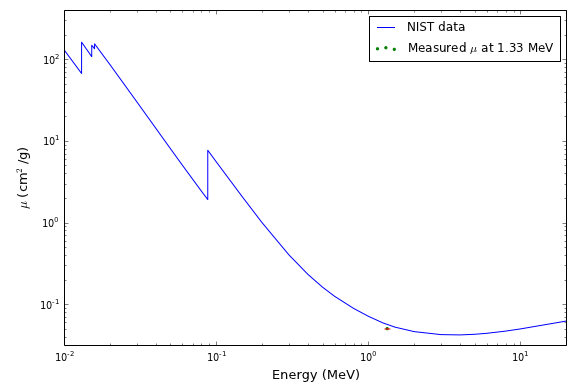
\includegraphics[width=.8\textwidth]{LeadMu.png}
\caption{The measured value for $\mu$ at 1.33 MeV compared against attenuation data from NIST\cite{NIST}.}
\label{LeadMu}
\end{figure}

\newpage

\subsection{Aluminum}

From the data in Table \ref{Trials}, $\alpha$ was determined to be $0.149\pm0.001$ cm$^{-1}$ using a fit function of the form of Eq \eqref{ln(I)} and the least squares method previously described. From this value we find $\lambda$ to be $6.70\pm0.05$ cm and $L_{1/2}$, the distance at which the intensity is reduced by a factor of 1/2, to be $4.64\pm0.03$ cm. Given that the density of aluminum is 2.7 g/cm$^3$, $\alpha$ also gives us a value for $\mu$ which is $0.0552\pm0.004$ cm$^2$/g. Again, NIST has no specific value for the attenuation coefficient at 1.33 MeV for aluminum. data extracted from Fig \ref{AluminumMu} gives an accepted value of 0.0535 cm$^2$/g showing that our value is in disagreement with what can be extrapolated from NIST's data \cite{NIST}.

\begin{figure}[h!]
\centering
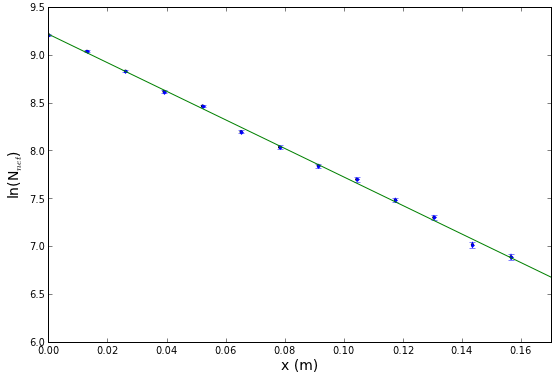
\includegraphics[width=.8\textwidth]{AluminumFit.png}
\caption{The least squares optimization of $\alpha$ and $ln(I_0)$ based on absorbent thickness and the natural log of the intensity.}
\label{AluminumFit}
\end{figure}

\begin{figure}[h!]
\centering
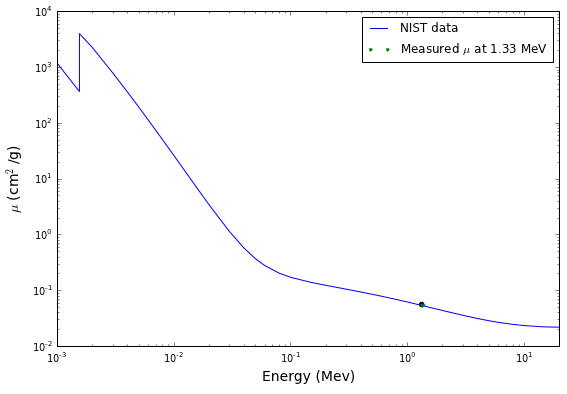
\includegraphics[width=.8\textwidth]{AluminumMu.png}
\caption{The measured value for $\mu$ at 1.33 MeV compared against attenuation data from NIST\cite{NIST}.}
\label{AluminumMu}
\end{figure}

\newpage

\section{Conclusion}

The purpose of this report was to quantitatively define the ability of gamma-rays to penetrate materials using the attenuation coefficient. By utilizing a PMT, MCA, and a scintillating NaI crystal, that coefficient was determined for a beam of gamma-rays emitted by a $^{60}$Co source. Given that the density of lead is 11.3 g/cm$^3$, and the density of aluminum is 2.7 g/cm$^3$, $\mu$, as found from lead, was $0.0501\pm0.0004$ cm$^2$/g, while its value as found from aluminum was $0.0552\pm0.0004$ cm$^2$/g. $\mu$ from lead is in disagreement with what can be extrapolated from data collected from NIST and $\mu$ from aluminum is in disagreement with NIST's data.

\newpage

\begin{acknowledgments}


\end{acknowledgments}


\begin{thebibliography}{99}

\bibitem{NIST} J. H. Hubbell, S. M. Seltzer, ``Tables of X-Ray Mass Attenuation Coefficients and Mass Energy-Absorption Coefficients from 1 keV to 20 MeV for Elements Z = 1 to 92 and 48 Additional Substances of Dosimetric Interest'' Radiation and Biomolecular Physics Division, PML, NIST, (1996).

\bibitem{henri} Henri Becquerel (1896). ``Sur les radiations �mises par phosphorescence". Comptes Rendus \textbf{122}: 420--421.

\bibitem{curie} Mould, R. F. (1998). ``The discovery of radium in 1898 by Maria Sklodowska-Curie (1867--1934) and Pierre Curie (1859--1906) with commentary on their life and times". The British Journal of Radiology \textbf{71} (852): 1229--54.

\bibitem{V1}Leif Gerward, Andr� Rassat, ``Paul Villard's discovery of gamma rays--A centenary, Comptes Rendus de l'Acad�mie des Sciences"Series IV,Volume 1, Issue 7, September 2000, pp. 965-973.

\bibitem{V2}Clarke, R.H.; and J. Valentin (2009). ``The History of ICRP". ICRP Publication 109 \textbf{39} (1): pp. 75--110

\end{thebibliography}

\end{document}
